
\chapter{Théorie algébrique des graphes}
\thispagestyle{empty}
\label{chap-theorie-algebrique-graphes} 

La référence principale sur la théorie spectrale des graphes est \cite{chung-spectral}. On pourra aussi consulter \cite{terras}.
%------------------------------------------------------
%------------------------------------------------------
%------------------------------------------------------
%		section -- Généralités
%------------------------------------------------------
%------------------------------------------------------
%------------------------------------------------------
\section{Généralités}
% \addcontentsline{toc}{section}{Généralités}
\label{sect1-theorie-graphes-généralites} 

Graphes, arrète, adjacence, structure de données (algorithmique des graphes).
%------------------------------------------------------
%------------------------------------------------------
%		sub-section -- Définitions
%------------------------------------------------------
%------------------------------------------------------
\subsection{Définitions}
\label{sect2-theorie-alg-graphes-dfn} 


%------------------------------------------------------
%------------------------------------------------------
%		sub-section -- Algorithmiques des graphes
%------------------------------------------------------
%------------------------------------------------------
\subsection{Algorithmiques des graphes}
\label{sect2-algorithmique-graphes} 

Plus court chemins (de 1 à tous, de tous à tous). Heuristique et distance euclidienne (algorithme A*). Problématique : introduire un peu d'algèbre pour résoudre certaines questions sur les propriétés des graphes. Comme pour la transformée de Fourier, on va étutidier un espace fonctionnel, celui des fonctions dont le domaine de départ est un graphe donné. Ceci va permettre d'une part d'analyser ces fonctions (en utilisant la structure du graphe), et d'autre part d'obtenir des informations sur le graphes. D'ailleur l'utilisation de la structure de graphe va rejoindre l'utilisation de la structure de groupe lors de l'étude des graphes de Cayley. L'étude spectrale des graphes peut donc être vue comme une généralisation de la transformée de Fourier sur un groupe fini.
%------------------------------------------------------
%------------------------------------------------------
%		sub-section -- Triangulations
%------------------------------------------------------
%------------------------------------------------------
\subsection{Triangulations}
\label{sect2-triangulations} 


\mathspace{}
\begin{defn}[Triangulation]

\end{defn}\noindent
La notion de triangulation permet de relier la notion de graphe à celle de surface. On parle ici d'une surface abstraite (c'est-à-dire au sens topologique), sans se préocuper de la réalisation géométrique de cette surface (ceci sera fait à la section \ref{sect1-representations-geometriques}). La figure \figref{fig-graph-examples-meshes} montre des exemples de triangulation. Pour les dessiner, on a placer chaque sommet dans $\RR^3$ (c'est par exemple le travail d'un artiste ou d'un infographiste). Cette représentation graphique serra précisée à la section \ref{sect1-representations-geometriques}.\begin{figure}[ht] 
    \begin{center}
    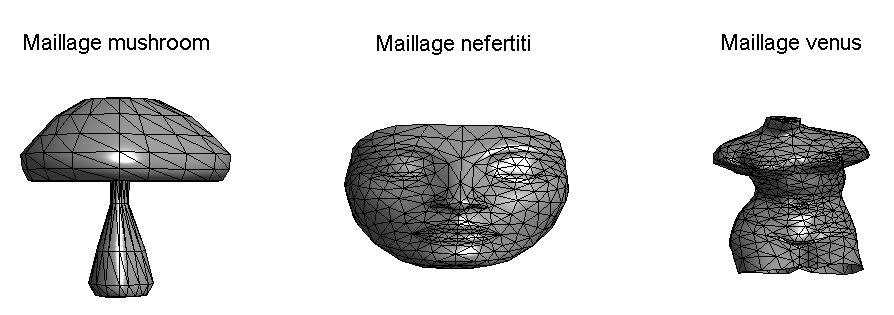
\includegraphics[scale=0.7]{images/graph-examples-meshes.eps}
    \end{center}
    \caption{Exemples de triangulations}
	 \label{fig-graph-examples-meshes}
\end{figure}

%------------------------------------------------------
%------------------------------------------------------
%------------------------------------------------------
%		section -- Théorie spectrale des graphes
%------------------------------------------------------
%------------------------------------------------------
%------------------------------------------------------
\section{Théorie spectrale des graphes}
% \addcontentsline{toc}{section}{Théorie spectrale des graphes}
\label{sect1-theorie-spectrale-graphes} 

Après cette introduction de nature combinatoire, qui a permis de fixer les notations, on va rentrer dans le vif du sujet, en s'intéressant à l'aspect algébrique des graphes. On va en particulier mettre en évidence les relations de parentés entre l'étude des fonctions sur un graphe et la théorie de Fourier sur un groupe fini.
%------------------------------------------------------
%------------------------------------------------------
%		sub-section -- Matrice d'adjacence et laplacien
%------------------------------------------------------
%------------------------------------------------------
\subsection{Matrice d'adjacence et laplacien}
\label{sect2-matrice-adjacence-laplacien} 


Comme dans tout le reste du livre, notre but est d'analyser des fonctions. Dans ce chapitre, on va étudier $\CC[\Gg]$ l'espace vectoriel des fonctions d'un graphe $\Gg$ dans $\CC$. Lorsque $G$ est un groupe fini, l'étude de $\CC[G]$ est grandement facilité par l'existence d'une base orthonormée \guill{adéquate}, en l'occurence celle des caractère, qui forme le groupe dual $\wh{G}$ (voir chapitre \ref{chap-transformee-fourier-groupe-fini}). Pour étudier $\CC[\Gg]$, on souhaite également exiber une base orthonormée qui respecte au maximum la structure de l'espace de départ des fonctions, c'est-à-dire la structure de graphe.

\paraspace
Sur les groupes finis, on a vu que les caractères sont les vecteurs propres des opérateurs de convolution. Par exemple pour $G = \ZZ/n\ZZ$, le plus simple est de considérer l'opérateur suivant
\begin{equation*}
\Ll_G : \func{ \CC[G] }{ \CC[G] } { f }{ f * a } \quad \text{où} \quad \left\{ \begin{array}{l} a[1] = a[-1] = 1/2, \\ a[0] = -1, \\ a[i] = 0 \quad \text{pour} \quad i \notin \{-1,\,0,\,1\}. \end{array} \right.
\end{equation*}
Cet opérateur est nommé \guill{Laplacien} car il correspond à une discrétisation de l'équation de la chaleur avec un pas temporel de 1 et un pas spacial de 1 (voir à ce propos l'exercice \oldref{exo-resol-eq-chaleur-diff-finies}). Ainsi, si on pose $T = \Id+\Ll_G, $$(T \circ \cdots \circ T)(f)$ correspond à une version \guill{lissée} de $f$, puisque c'est une approximation (certes grossière) de l'équation de la chaleur (définie en \ref{sect2-resol-eq-chaleur}) avec comme condition initiale $f$. La figure \figref{} montre cet effet de lissage.

\paraspace
Pour définir une base orthonormée de $\CC[\Gg]$, il est donc naturel d'introduire un opérateur similaire (c'est-à-dire de lissage), que l'on nommera Laplacien du graphe $\Gg$.
\mathspace{}
\begin{defn}[Laplacien d'un graphe]
\label{defn-laplacien-graphe}

\end{defn}\noindent

\mathspace{}
\begin{prop}[Propriété du Laplacien]
\label{prop-laplacien-graphe}
Parler du PageRank de Google, qui utilise les vecteurs propres du Laplacien. Dire intuitivement ce que l'on veut faire : placer les sites internet sur une droite, en prenant en compte les liens qui les relie.
\end{prop}\noindent

%------------------------------------------------------
%------------------------------------------------------
%		sub-section -- Transformée de Fourier sur un graphe
%------------------------------------------------------
%------------------------------------------------------
\subsection{Transformée de Fourier sur un graphe}
\label{sect2-transfo-fourier-graphe} 

Définition des vecteurs propres, et de l'espace des fonction de $\Gg \rightarrow \CC$. Donner des exemples "graphiques", dire que l'on parlera de la façon de représenter un graphe à la section suivante, mais que pour l'instant on dessine un graphe en plaçant ses sommets dans le plan "le mieux possible".
\mathspace{}
\begin{rem} {(\upshape\textbf{Graphe et recherche sur internet}).} 

\end{rem}\noindent

%------------------------------------------------------
%------------------------------------------------------
%------------------------------------------------------
%		section -- Graphes de Cayley
%------------------------------------------------------
%------------------------------------------------------
%------------------------------------------------------
\section{Graphes de Cayley}
% \addcontentsline{toc}{section}{Graphes de Cayley}
\label{sect1-graphes-cayley} 

En fait, la définition des vecteurs propres d'un graphe généralise celle des caractères sur un groupes finis commutatif. On va en effet construire, pour un groupe $G$ donné, une famille de graphes ayant tous les même vecteurs propres, qui sont justement les caractères du groupe. En quelque sorte, pour ces graphes, la symétrie induite par la structure de groupe est la même que celle induite par la structure de graphe.
%------------------------------------------------------
%------------------------------------------------------
%		sub-section -- Définition
%------------------------------------------------------
%------------------------------------------------------
\subsection{Définition}
\label{sect2-graphe-cayley-defn} 


\mathspace{}
\begin{defn}[Graphe de Caley]

\end{defn}\noindent
Faire le lien entre le graphe cyclique et la TFD.
%------------------------------------------------------
%------------------------------------------------------
%		sub-section -- Exemples de graphes de Cayley
%------------------------------------------------------
%------------------------------------------------------
\subsection{Exemples de graphes de Cayley}
\label{sect2-exmp-cayley} 


%------------------------------------------------------
%------------------------------------------------------
%		sub-section -- Marches aléatoires
%------------------------------------------------------
%------------------------------------------------------
\subsection{Marches aléatoires}
\label{sect2-marches-aleatoires} 


%------------------------------------------------------
%------------------------------------------------------
%------------------------------------------------------
%		section -- Représentations géométriques des graphes
%------------------------------------------------------
%------------------------------------------------------
%------------------------------------------------------
\section{Représentations géométriques des graphes}
% \addcontentsline{toc}{section}{Représentations géométriques des graphes}
\label{sect1-representations-geometriques} 

Dans cette section, on va chercher des fonctions d'un graphe $\Gg$ dans $\RR^n$ ayant des propriétés intéressantes. Une fois de plus, on va voir que l'analyse des signaux (ici de $\Gg$ dans $\RR$) a une nature géométrique, et on pourra rapprocher cette étude de celle faite à la section \ref{sect1-aspect-geometriques} sur les polygones. On va voir que cette étude géométrique permet d'obtenir des informations extrèmement \guill{visuelles} sur un graphe.
%------------------------------------------------------
%------------------------------------------------------
%		sub-section -- Réalisation géométrique
%------------------------------------------------------
%------------------------------------------------------
\subsection{Réalisation géométrique}
\label{sect2-realisation-geometrique} 



\mathspace{}
\begin{defn}[Réalisation géométrique]
Une réalisation géométrique d'un graphe $\Gg = (S,\,A)$ est la donnée d'une fonction $F : S \rightarrow\RR^n$, qui \guill{place} chaque sommet de $\Gg$. Par abus de notation, on notera aussi $F : \Gg \rightarrow \RR^n$.
\end{defn}\noindent


\paraspace
Si le graphe est associé à une triangulation, alors une réalisation géométrique permet de définir une surface de dimension 2. Typiquement, les figure \figref{fig-graph-examples-meshes} et \ref{fig-graph-examples-meshes-normal} on été réalisée en utilisant des réalisation dans $\RR^3$, ce qui permet d'obtenir des dessins 3D de surfaces. On peut même définir des normales pour chaque sommet, comme le montre la figure \figref{fig-graph-examples-meshes-normal}. Si on ne dispose pas à priori de ces normales, on peut les calculer en chaque sommet en réalisant la moyenne des normales aux faces adjacentes, ou en employant des méthodes plus complexes \cite{cohen-normal-cycles}.\begin{figure}[ht] 
    \begin{center}
    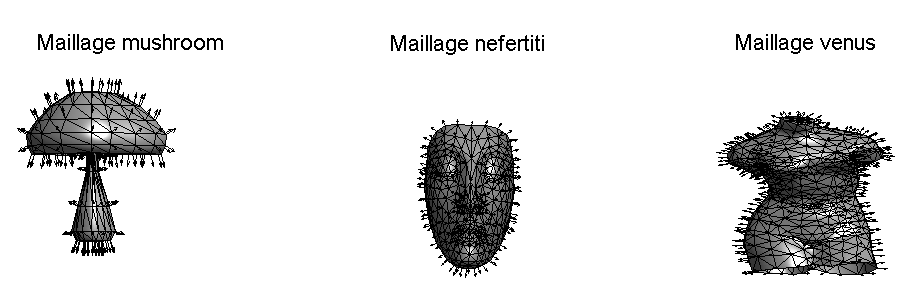
\includegraphics[scale=0.7]{images/graph-examples-meshes-normal.eps}
    \end{center}
    \caption{Exemples de triangulations}
	 \label{fig-graph-examples-meshes-normal}
\end{figure}


\paraspace
On a déjà fait remarquer que l'opérateur $T = \Id+\Ll_\Gg$ permetait de réaliser un lissage d'une fonction $f \in \CC[\Gg]$ définie sur un graphe. En considérant une réalisation géométrique $F : \Gg \rightarrow \RR^n$ comme une collection de $n$ fonctions $F \eqdef (f_1,\ldots,\,f_n)$, on peut appliquer l'opérateur $T$ à chaque $f_i \in \CC[\Gg]$. On obtient ainsi un lissage de la représentation, et en considérant une triangulation, un lissage de la surface sous-jacente. C'est ce que montre la figure \figref{fig-graph-smoothing} pour plusieurs itérations du lissage, à partir d'une triangulation déformée (on a ajouté un bruit selon la direction de la normale à chaque sommet).\begin{figure}[ht] 
    \begin{center}
    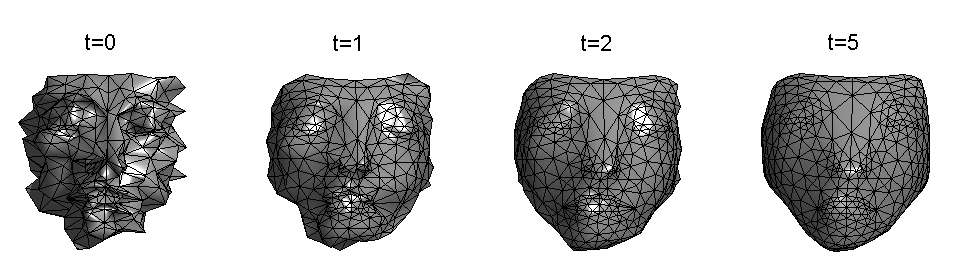
\includegraphics[scale=0.7]{images/graph-smoothing.eps}
    \end{center}
    \caption{Lissage d'un maillage à l'aide de Laplacien}
	 \label{fig-graph-smoothing}
\end{figure}

%------------------------------------------------------
%------------------------------------------------------
%		sub-section -- Dessiner un graphe
%------------------------------------------------------
%------------------------------------------------------
\subsection{Dessiner un graphe}
\label{sect2-dessiner-graphe} 


Le but de cette section, est, étant donné un graphe, de trouver trouver une réalisation géométrique $F : \Gg \rightarrow \RR^2$ d'un graphe $\Gg = (S,\,A)$. On va d'abord étudier le problème en toute généralité, puis voir comment on peut exploiter des informations supplémentaires pour améliorer cette réalisation géométrique.

\paraspace
Le but est donc de trouver une placement le plus \guill{harmonieux} possible des sommets du graphe pour que ce dernier soit plus facile à comprendre. Il est donc naturel de placer proches les uns des autres des sommets qui sont reliés par des arrètes. On introduit alors une énergie qui mesure combien une réalisation $F$ est correcte
\begin{equation*}
E(F) \eqdef \sum_{i \in A}{ \sum_{j \sim i}{ w_{i,j} \norm{ F(i)-F(j) }^2 } },
\end{equation*}
où les $w_{i,j}$ sont des poids à déterminer, qui vérifient $w_{i,j} = w_{j,i}$. Bien sûr, si l'on ne place pas d'autre condition sur $F$, il n'y a aucune chance que cette méthode aboutisse, puisqu'il suffit de choisir $F$ qui envoit tous les sommets sur un même point pour avoir $E(F)=0$. On va donc chercher $\wt{F}$ qui vérifie
\begin{equation*}
\left\{ \begin{array}{ll} \wt{F} = \text{argmin}_{F}( E(F) ), \quad \text{avec} & \\ \sum_{i \in S}{F(i)}=0 & (C_1), \\ \sum_{i \in S}{F(i)^2}=0 & (C_2). \end{array} \right.
\end{equation*}
La condition $(C_1)$ oblige le dessin à être centré à l'origine, et la condition $C_2$ oblige les sommets à être bien répartis autour de $0$. Il est facile de voir que si $\wt{F}$ est solution du problème, alors tout dessin obtenu par rotation autour de $0$ du dessin d'origine est encore solution. Pour un graphe générique, c'est en fait le seul degrés de liberté dans l'espace des solutions. Par abus de notations, on va noter $F = (f_1,\,f_2)$ et on va encore noter $f_1,\,f_2 \in \RR^{n_V}$, où $n_V = \#V$, les vecteurs $\{f_1(i)\}_{i \in V}$ et $\{f_2(i)\}_{i \in V}$.

\paraspace
Si on prend comme choix de poids
\begin{equation*}
w_{i,j} = TODO
\end{equation*}
alors on voit que les vecteurs $f_1$ et $f_2$ sont les vecteurs propres du Laplacien combinatoire $\Ll_\Gg$ du graphe. La figure \ref{fig-graph-drawing-triangulation} (en haut à gauche), montre un dessin obtenu par cette méthode pour une triangulation. Ceci correspond bien à réaliser un \guill{applatissement} de la surface 3D d'origine.\begin{figure}[ht] 
    \begin{center}
    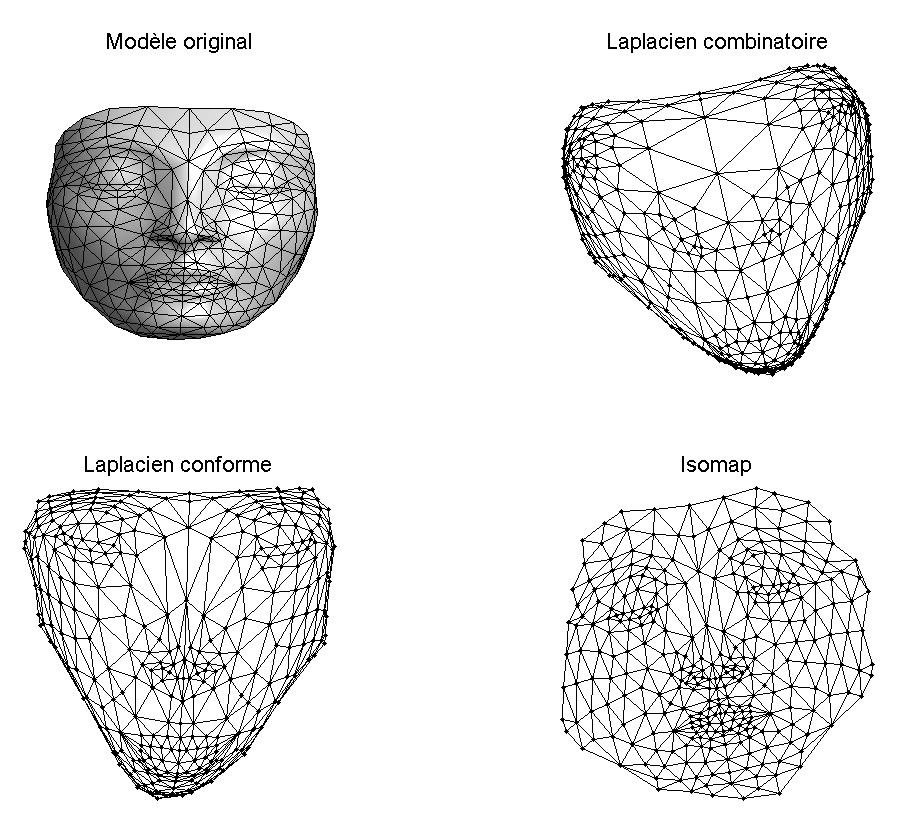
\includegraphics[scale=0.6]{images/graph-drawing-triangulation.eps}
    \end{center}
    \caption{Dessin d'une triangulation par 3 méthodes}
	 \label{fig-graph-drawing-triangulation}
\end{figure}


\paraspace
Le dessin obtenu avec le Laplacien combinatoire est correct, mais il ne tient pas compte de la surface 3D dont on disposait au départ. En effet, on n'a exploiter que la connectivité du graphe, ce qui montre que cette méthode est très puissante pour dessiner des graphes \guill{abstraits}, mais elle est insufisante si l'on dispose d'une réalisation particulière $F : \Gg \rightarrow \RR^3$ de la surface. Dans le but d'exploiter la géométrie de la surface, les auteurs de \cite{alliez-parameterization} ont proposé comme poids
\begin{equation*}
w_{i,j} = \sum_{ j \sim i }{ \left( \text{cot}(\alpha_{i,j})+\text{cot}(\beta_{i,j}) \right) },
\end{equation*}
où les angles $\alpha_{i,j}$ et $\beta_{i,j}$ sont définis à la figure \figref{}. Ces poids portent le nom de \guill{poids conformes}, car il visent à minimiser une énergie qui s'inspire de la théorie de la représentation conforme. La matrice $L$ correspondant s'appelle donc Laplacien conforme. La figure \ref{graph-drawing-triangulation}, en bas à gauche, montre le résultat d'un dessin obtenu par cette méthode, et on observe une bien meilleure conservation de la géométrie de la surface.

\paraspace
Parler d'IsoMap.
%------------------------------------------------------
%------------------------------------------------------
%		sub-section -- Paramétrer une triangulation
%------------------------------------------------------
%------------------------------------------------------
\subsection{Paramétrer une triangulation}
\label{sect2-parametrer-triangulation} 


Dans cette partie, on va considérer une rafinement du problème de dessin de graphe abordé à la section précédente. On souhaite en effet que lorsque l'on dessine les arrètes de la réalisation géométrique dans $\RR^2$, aucune d'entre-elles ne se touche. Il est évident que sur un graphe générique, un tel dessin est impossible à réaliser. Les graphes pour lesquels on peut faire un tel dessin sont nommés \textit{graphe planaires}.

\paraspace
Dans la suite, on va se restreindre aux graphes correspondant à des triangulations. On va de plus supposer que l'on dispose d'une triangulation topolgiquement équivalente à un disque. De façon intuitive, ceci signifie qu'il n'y a pas de \guill{trou} dans la triangulation.

\paraspace
\begin{figure}[ht] 
    \begin{center}
    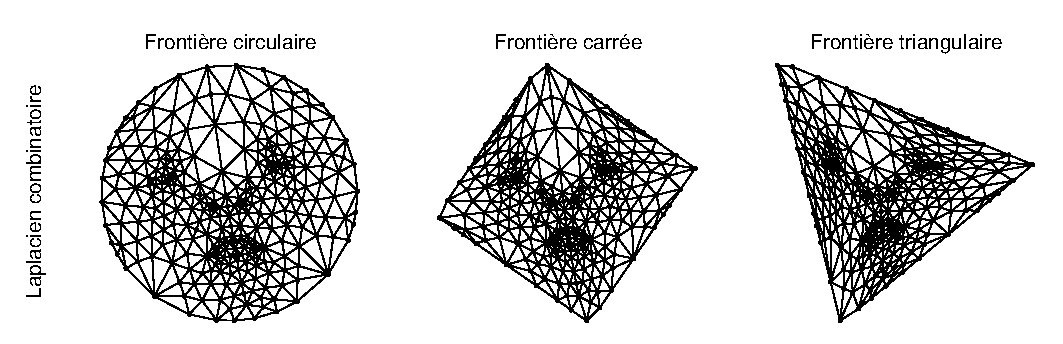
\includegraphics[scale=0.6]{images/graph-parameterization-1.eps}
    \includegraphics[scale=0.6]{images/graph-parameterization-2.eps}
    \end{center}
    \caption{Exemples de paramétrisations d'un maillage}
	 \label{fig-graph-parameterization}
\end{figure}

%------------------------------------------------------
%------------------------------------------------------
%		sub-section -- Compression de maillage
%------------------------------------------------------
%------------------------------------------------------
\subsection{Compression de maillage}
\label{sect2-compression-maillage} 

\begin{figure}[ht] 
    \begin{center}
    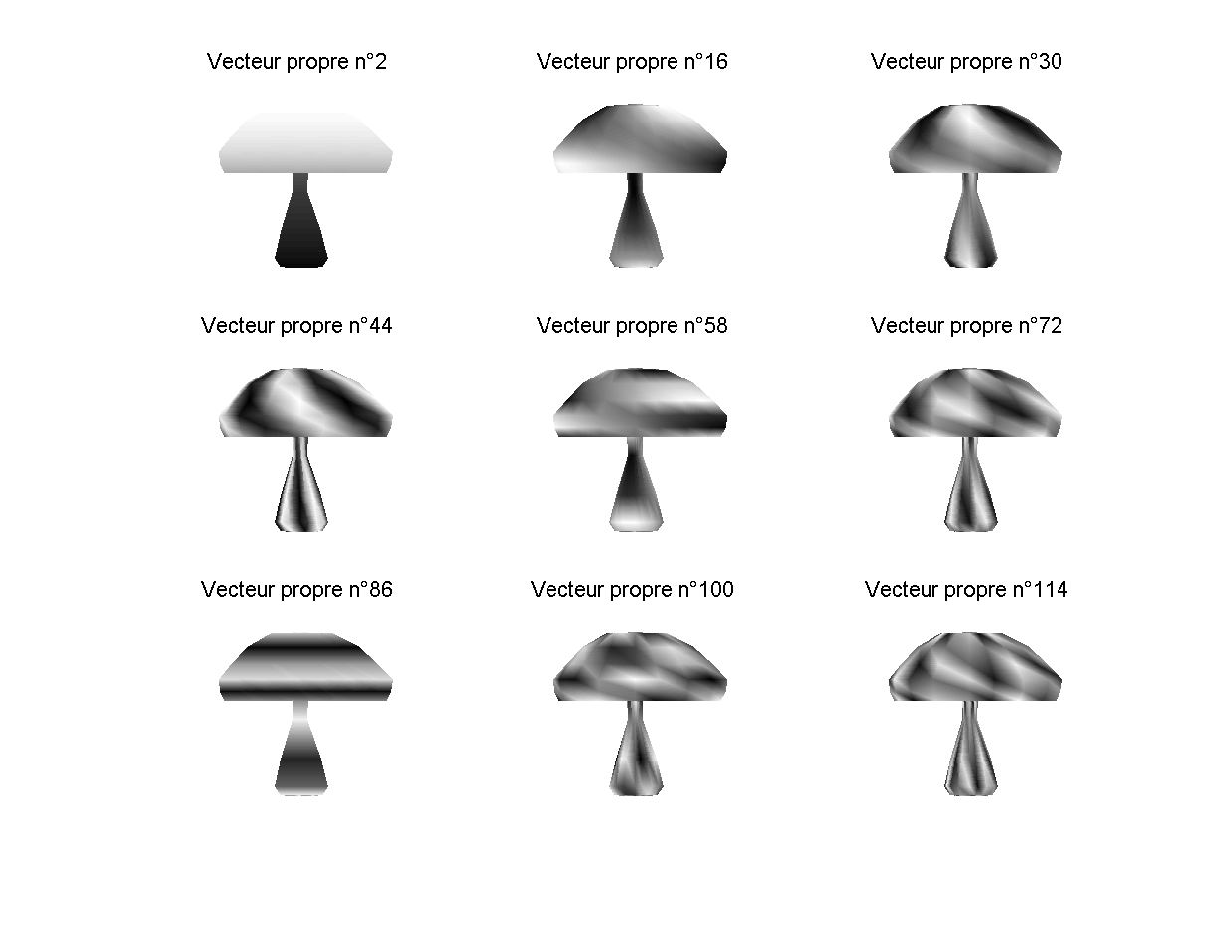
\includegraphics[scale=0.6]{images/graph-compression-eigenvectors.ps}
    \end{center}
    \caption{Vecteurs propres du Laplacien}
	 \label{fig-graph-compression-eigenvectors}
\end{figure}
\begin{figure}[ht] 
    \begin{center}
    \includegraphics[scale=0.6]{images/graph-compression-progression.eps}
    \end{center}
    \caption{Compression progressive du modèle du champignon}
	 \label{fig-graph-compression-progression}
\end{figure}

%------------------------------------------------------
%------------------------------------------------------
%------------------------------------------------------
%		section -- Exercices
%------------------------------------------------------
%------------------------------------------------------
%------------------------------------------------------
\section{Exercices}
% \addcontentsline{toc}{section}{Exercices}
\label{sect1-chap2-exercices} 


\mathspace{}
\begin{exo}[Schémas de subdivision]
\label{exo-schemas-subdivision}

Introduire ici les schéma de subdivision 1:4.\begin{figure}[ht] 
    \begin{center}
    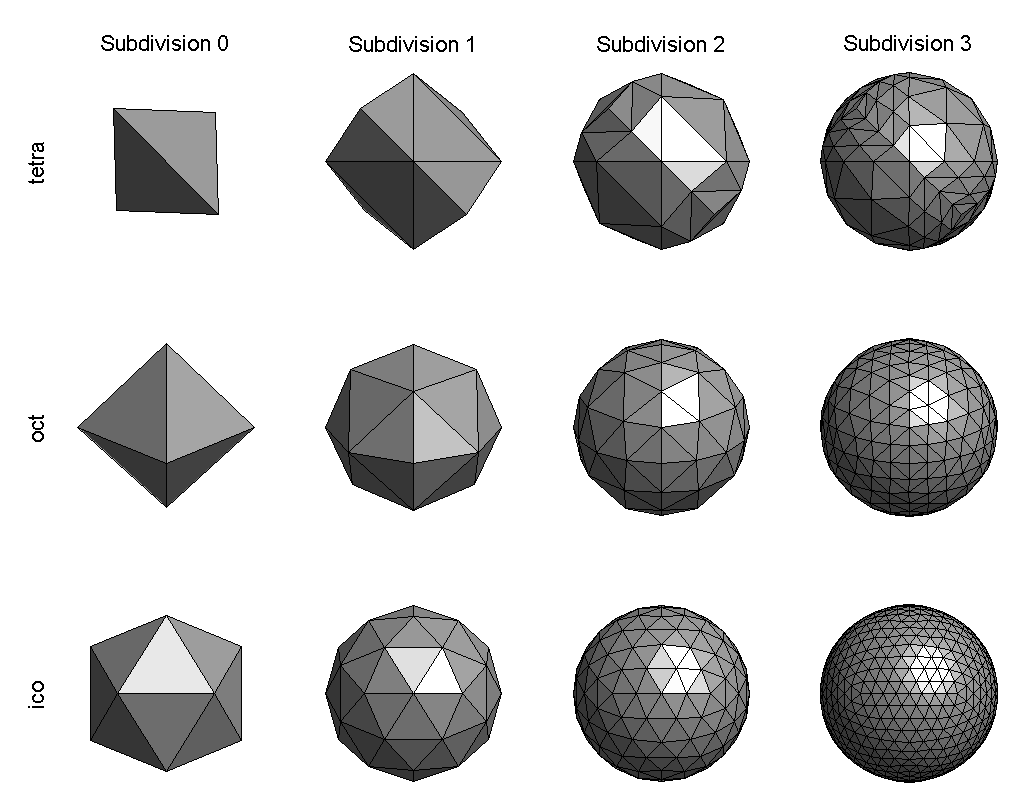
\includegraphics[scale=0.6]{images/graph-subdivision-sphere.eps}
    \end{center}
    \caption{Subdivision successive d'un icosaèdre}
	 \label{fig-graph-subdivision-sphere}
\end{figure}
\begin{figure}[ht] 
    \begin{center}
    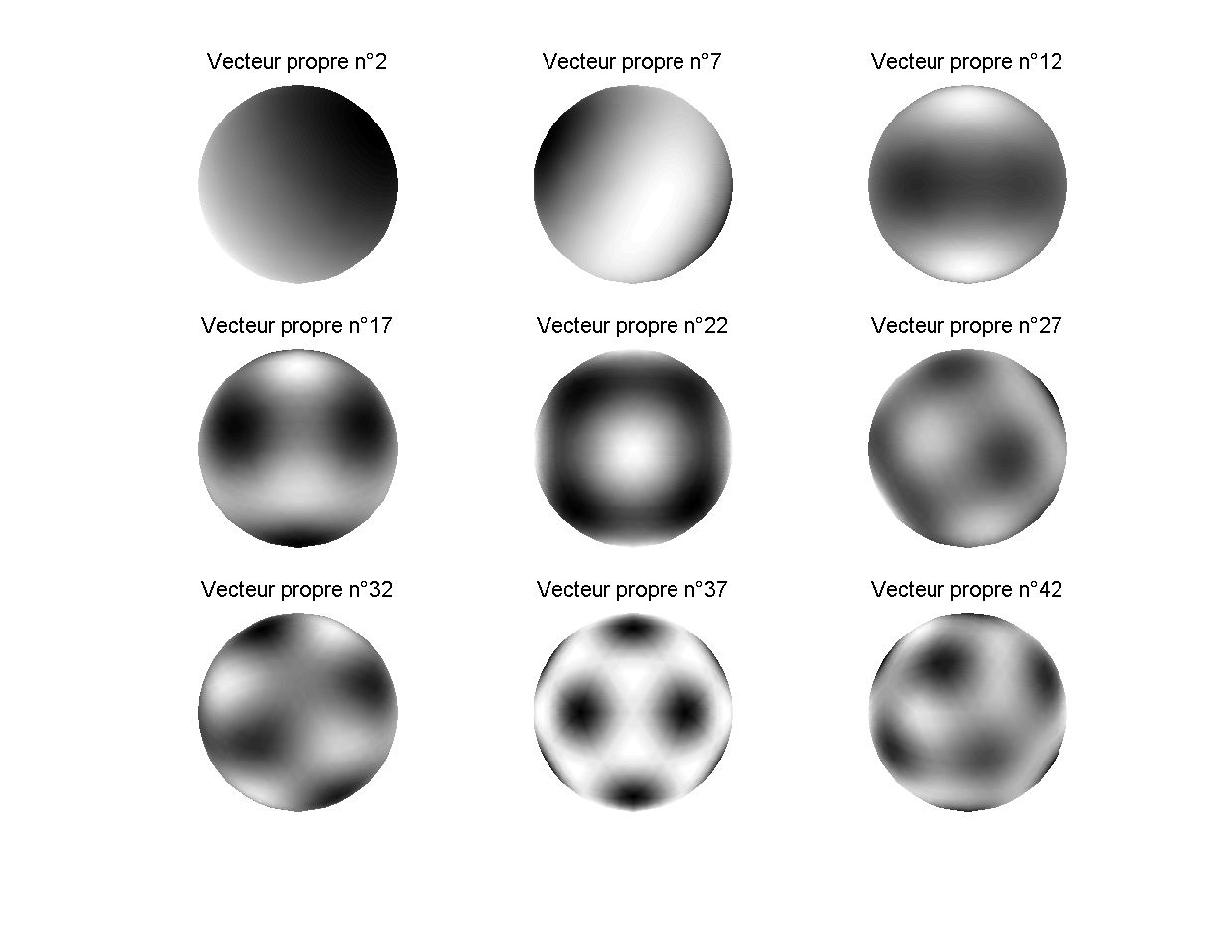
\includegraphics[scale=0.6]{images/graph-subdivision-vecteurs-propres.ps}
    \end{center}
    \caption{Vecteurs propres du Laplacien sur une sphère subdivisée}
	 \label{fig-graph-subdivision-vecteurs-propres}
\end{figure}

\end{exo}\noindent

